\section{Integration Strategy}
\subsection{Entry Criteria}
	Before starting the test phase the following doucments must be ready and read:
	\begin{itemize}
		\item The Design Document of previous delivery to understand how the software is built. In particular the component view which specifies how the various modules of the system are connected to each other.
		\item Sections 2.3 and 2.4 of this document that explains which explains which strategy we use and the testing order of every module and submodule.
		\item How the database is built and which data it contains
		
		Also before testing each module that comes after some other module in the testing order:
		
		\item Test result of previous order and the drivers required to run that test
	\end{itemize} 
\subsection{Elements to be Integrated}
		\begin{center}
			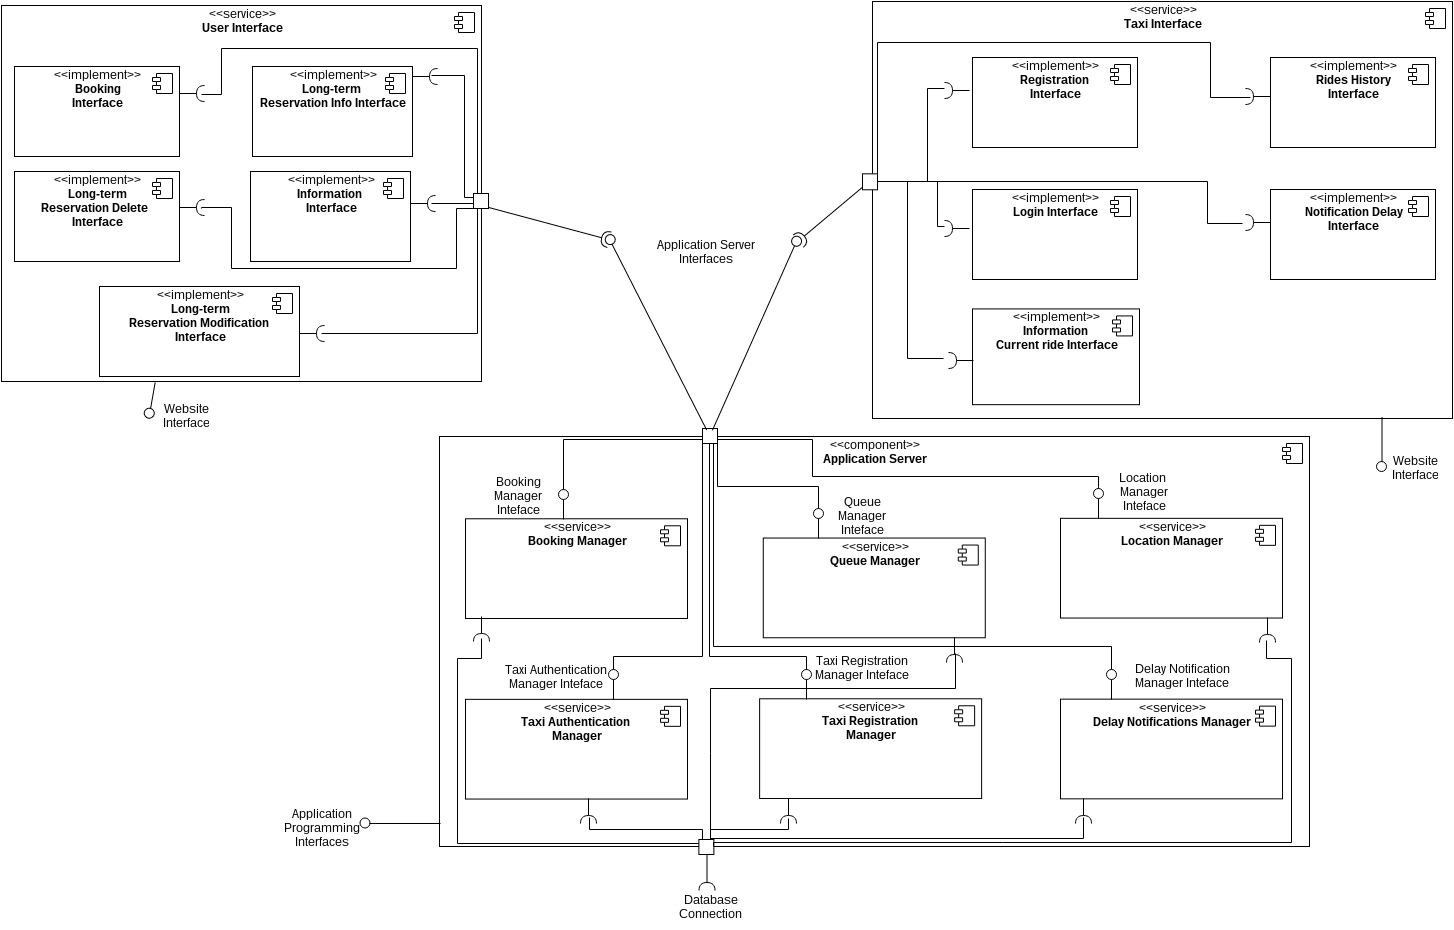
\includegraphics[width=0.95\textwidth]{./images/test_modules.png}
		\end{center}
		The system to be tested is represented in this image. Every submodule has to be tested after all his predecessors in testing order, specified in section 2.5, have been tested. The system can be divided in 3 modules, and every module can be divided in submodules.
		\newline
		\newline
		\noindent \textbf{Modules to be Tested}
		
		\begin{itemize}
			\item \textbf{Application Server}
			\begin{itemize}
				\item Booking Manager
				\item Taxi Authentication Manager
				\item Queue Manager
				\item Taxi Registration Manager
				\item Location Manager
				\item Delay Notification Manager
			\end{itemize}
			\item \textbf{Taxi Interface}
			\begin{itemize}
				\item Registration Interface
				\item Login Interface
				\item Information Current Ride Interface
				\item Rides History Interface
				\item Notification Delay Interface
			\end{itemize}
			\item \textbf{User Interface}
			\begin{itemize}
				\item Booking Interface
				\item Long-term Reservation Delete Interface
				\item Long-term Reservation Info Interface
				\item Information Interface
				\item Long-term Reservation Modification Interface
			\end{itemize}
		\end{itemize}
\subsection{Integration Testing Strategy}
\subsection{Sequence of Component/Function Integration}
\subsubsection{Software Integration Sequence}
\subsubsection{Subsystem Integration Sequence}